\documentclass[a4paper,10pt]{article}

\usepackage[utf8]{inputenc}
\usepackage{t1enc}

\usepackage[utf8]{inputenc}
\usepackage{t1enc}
\usepackage[spanish]{babel}
\usepackage[pdftex,usenames,dvipsnames]{color}
\usepackage[pdftex]{graphicx}
\usepackage{enumerate}
\usepackage{amsmath}
\usepackage{amsfonts}
\usepackage{amssymb}
\usepackage[table]{xcolor}
\usepackage[small,bf]{caption}
\usepackage{float}
\usepackage{subfig}
\usepackage{listings}
\usepackage{bm}
\usepackage{times}

\begin{document}

\renewcommand{\lstlistingname}{C\'odigo Fuente}
\lstloadlanguages{Octave} 
\lstdefinelanguage{MyOctave}[]{Octave}{
	deletekeywords={beta,det},
	morekeywords={repmat}
} 
\lstset{
	language=MyOctave,
	stringstyle=\ttfamily,
	showstringspaces = false,
	basicstyle=\footnotesize\ttfamily,
	commentstyle=\color{gray},
	keywordstyle=\bfseries,
	numbers=left,
	numberstyle=\ttfamily\footnotesize,
	stepnumber=1,                   
	framexleftmargin=0.20cm,
	numbersep=0.37cm,              
	backgroundcolor=\color{white},
	showspaces=false,
	showtabs=false,
	frame=l,
	tabsize=4,
	captionpos=b,               
	breaklines=true,             
	breakatwhitespace=false,      
	mathescape=true
}

%%%%%%%%%%%%%%%%%%%%%%%%%%%%%%%%%%
%%%%%%%% begin TITLE PAGE %%%%%%%%
%%%%%%%%%%%%%%%%%%%%%%%%%%%%%%%%%%
\begin{titlepage}
	\vfill
	\thispagestyle{empty}
	\begin{center}
		
\includegraphics{./images/itba.jpg}
		\vfill
		\Huge{EAC 2}\\
		\vspace{1cm}
		\Huge{Probabilidad y Estad\'istica}\\
	\end{center}
	\vfill
	\large{
        \begin{tabular}{lcr}
		De Elias, Miguek && 50457 \\
		Ordano, Esteban && 50753 \\
                Crespo, Alvaro && 50758 \\
        \end{tabular}
}
	\vspace{2cm}
	\begin{center}
		\large{26 de mayo de 2011}\\
	\end{center}
\end{titlepage}
\newpage

\section*{Enunciado}
En la caminata aleatoria o \textit{random walk} (\'o \textit{camintata del borracho}) unidimensional (\'o 1D) se considera el movimiento en una dimensi\'on 
(a lo largo de una l\'inea recta) de un punto que ocupa posiciones de abscisa entera. En cada instante (consideramos intervalos regulares) el punto se mueve a la derecha  (incrementando
su posici\'on en una unidad) con probabilidad $p$ \'o hacia la izquierda con probabilidad (1 - $p$), en este caso la coordenada de posici\'on se reduce en unidad.
\\ Si se asume que el movimiento es 2D entonces las coordenadas $x$ e $y$ se consideran enteras y en cada instante a partir de la posici\'on con coordenadas ($x$,$y$) con 
distribuci\'on uniforme la pr\'oxima posici\'on puede tomar uno de estos 4 valores: ($x+ 1$,$y$),($x- 1$,$y$),($x$,$y+1$) \'o ($x$,$y-1$). En la versi\'on 3D las coordenadas $x$, $y$ y $z$
se consideran enteras y en cada instante a partir de la posici\'on con coordenadas ($x$,$y$,$z$) y con distribuci\'on uniforme la pr\'oxima posici\'on puede tomar uno de estos 6 valores:
 ($x+ 1$,$y$, $z$),($x- 1$,$y$,$z$),($x$,$y+1$,$z$), ($x$,$y-1$,$z$), ($x$,$y$,$z+1$) \'o ($x$,$y$,$z-1$) .
\\ Suponga que $p = 0.5$ en el caso 1D y que la posici\'on inicial en cualquiera de los casos es el origen de coordenadas.
\\
\begin{enumerate}[a)]
\item Estime la probabilidad de la \textit{vuelta a casa} en la caminata aleatoria 1D sim\'etrica ($p=0.5$) por medio de una simulaci\'on. Considere el transcurso del tiempo 
(\textit{paso a paso}) hasta que la coordenada de posici\'on vuelva a valer cero. Suponga como m\'aximo un n\'umero grande de posibles transiciones para creer en el no retorno (por ejemplo
10000 pasos). Considere un n\'umero grande de pruebas ( tambi\'en 10000 \'o m\'as). Con la informaci\'on disponible estime la probabilidad pedida y tambi\'en el n\'umero promedio de pasos hasta la vuelta. Haga un histograma para el n\'umero de pasos.
\\ Tome alguna trayectoria (sucesi\'on de posiciones) que haya resultado \textit{larga} hasta que se produce el retorno (tal vez limitando el n\'umero m\'aximo de pasos considerado) y 
repres\'entela con la posici\'on y el tiempo como las coordenadas de un gr\'afico de dispersi\'on.
\\
\item  Estime la probabilidad de la \textit{vuelta a casa} en la caminatas aleatorias 2D y 3D por medio de una simulaci\'on. Considere el transcurso del tiempo (\textit{paso a paso}) 
hasta que la coordenada de posici\'on vuelva a ser el vecto nulo. Suponga como m\'aximo un n\'umero grande de posibles transiciones para creer en el no retorno (por ejemplo
10000 pasos). Tome alguna trayectoria (sucesi\'on de posiciones) que haya resultado \textit{larga} y repres\'entela en 2D para la caminata 2D y en 3D para la otra.
\end{enumerate}
Algunas referencias de recomendable consulta para poder entender algo de lo que vaya a observar en la simulaci\'on:
\begin{enumerate}
\item http://mathworld.wolfram.com/RandomWalk1-Dimensional.html
\item http://mathworld.wolfram.com/RandomWalk2-Dimensional.html
\item http://mathworld.wolfram.com/RandomWalk3-Dimensional.html
\item http://mathserver.sdu.edu.cn/mathency/math/p/p447.htm
\end{enumerate}
\newpage

\section{Punto A} 
Utilizando el c\'odigo del ap\'endice \ref{CodeC} (con dim = 1), para la caminata aleatoria 1D, y considerando un n\'umero de pasos igual a 10000 y 
de simulaciones igual a 10000, los resultados obtenidos fueron:
\\
\\  Probabilidad de la \text{vuelta a casa}: 0.9914.
\\  Promedio pasos hasta la vuelta: 75.55.
\\
\\ A continuaci\'on se muestra el histograma para el n\'umero de pasos. En \'el se puede observar la cantidad de simulaciones que 
lograron volver exitosamente para cada grupo de n\'umero de pasos.
\begin{center}
  \begin{figure}[H]
  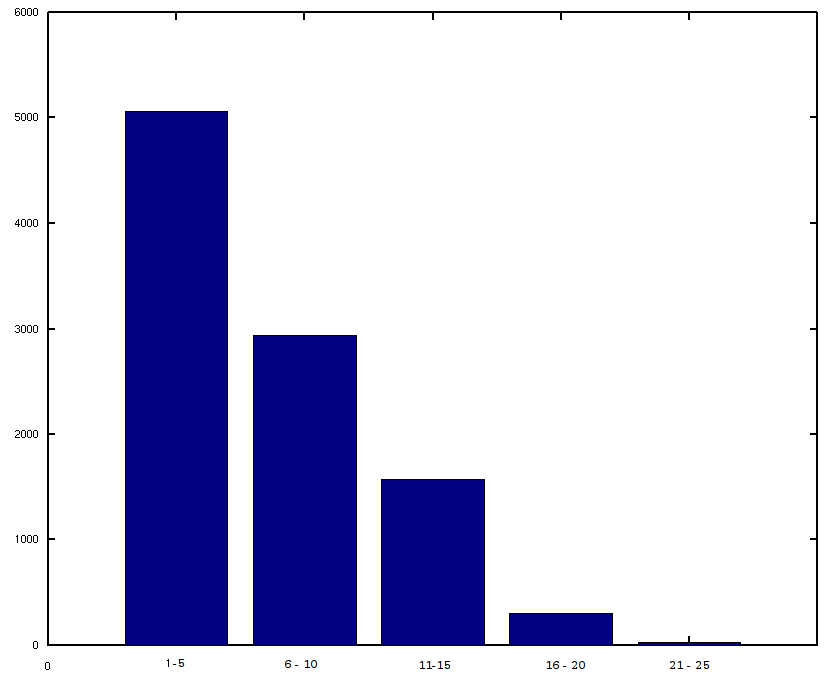
\includegraphics[scale=0.5]{./images/bar1edit.png}
    \caption{Histograma}
  \end{figure}
\end{center}
En la siguiente figura, se puede ver la trayectoria de una de las caminatas aleatorias que logr\'o exitosamente volver al origen.
\begin{center}
  \begin{figure}[H]
  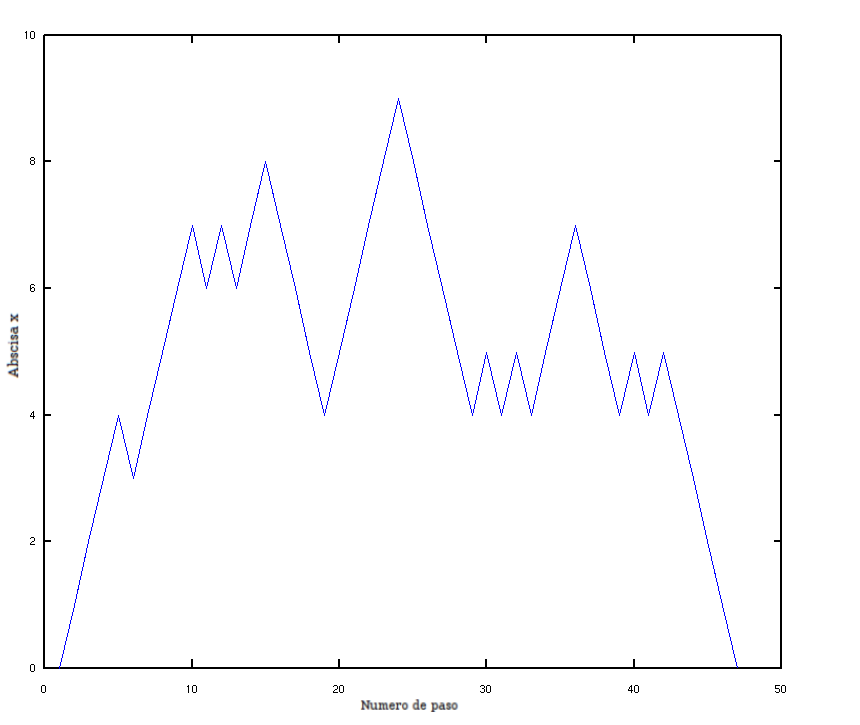
\includegraphics[scale=0.5]{./images/rec1edit.png}
    \caption{Trayectoria de una caminata aleatoria 1D}
  \end{figure}
\end{center} 
\newpage
\section{Punto B}
\subsection*{Caminata aleatoria 2D}
Para la caminata aleatoria 2D, utilizando de nuevo el mismo c\'odigo del ap\'endice \ref{CodeC} (esta vez con dim = 2), y considerando
 un n\'umero de pasos igual a 10000 y de simulaciones igual a 10000, los resultados obtenidos fueron:
\\
\\ Probabilidad de la \text{vuelta a casa}: 0.7350.
\\ Promedio de pasos hasta la vuelta: 366.49.
\\
\\ En la siguiente figura, se puede ver la trayectoria de una de las caminatas aleatorias que logr\'o exitosamente volver a casa.
\begin{center}
  \begin{figure}[H]
  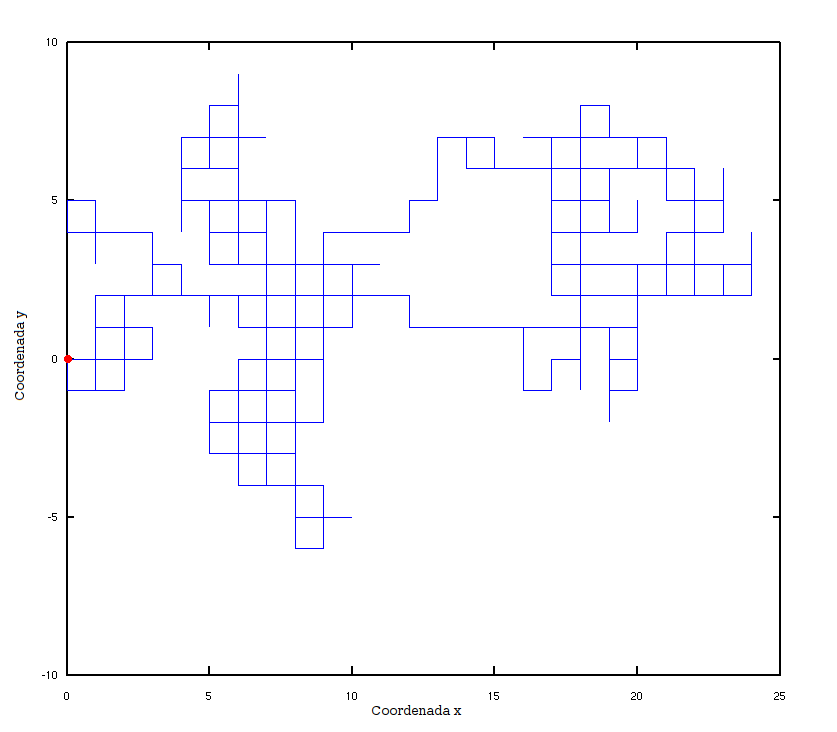
\includegraphics[scale=0.5]{./images/rec2edit.png}
    \caption{Trayectoria de una caminata aleatoria 2D}
  \end{figure}
\end{center} 
\subsection*{Caminata aleatoria 3D}
Para la caminata aleatoria 3D si se considera un n\'umero de pasos igual a 10000 y de simulaciones igual a 10000, el c\'odigo que 
se escribi\'o para Octave no era suficientemente r\'apido (se estimó que, dado que una caminata de 10000 pasos en la computadora
utilizada demoraba entre $3$ y $4$ segundos, $10000$ iteraciones demorar\'ian alrededor de 7 horas), se procedi\'o a realizar la
implementación de la caminata en el lenguaje de programaci\'on C, caracterizado por su eficiencia y el gran control que se tiene 
sobre las variables y el procesador.

De este modo, se pudieron realizar las siguientes optimizaciones:
\begin{itemize}
	\item \textbf{Diferencia entre lenguaje compilado (C) e interpretado (Octave)}. Al ser un lenguaje compilado, la ejecución del 
	c\'odigo es directa y no hay intermediarios analizando qu\'e es lo que se debe ejecutar. El c\'odigo escrito en Octave no es
	ejecutable, si no que el int\'erprete Octave hace un an\'alisis en tiempo real de los c\'odigos fuentes de Octave para luego
	decirle al microprocesador qu\'e operaciones realizar.
	\item \textbf{Pasaje de resultados por variables globales}. Al declarar las funciones de manera global, se evita el copiado 
	entre una funci\'on y otra de los resultados obtenidos.
	\item \textbf{Evitar arreglos de tamaño variable}. Al no utilizar arreglos de tamaño variable, se ahorró tiempo considerable de 
	ejecución por evitar los pasos de reservar memoria, liberarla, pasos del recolector de basura, entre otros.
	\item \textbf{Declaraci\'on de funciones \textit{inline}}. Una funci\'on inline en el momento de ser compilada, es insertada
	autom\'aticamente dentro de la o las funciones que la llamen. Esto ahorra nanosegundos para el procesador, que se evita de 
	realizar el $"$armado de stack$"$, pero permite al compilador realizar varias optimizaciones que no le son evidentes en otro caso.
\end{itemize}

Algo que se debe aclarar es que la funci\'on $rand()$ de C no retorna un n\'umero de punto flotante, si no que retorna un entero.
Debido a esto, se tuvo que realizar un \textit{parche} para obtener un n\'umero aleatorio entre 1 y 3 (ver la funci\'on $realrand()$ en
\ref{CodeC}), que consistió en saltear dos valores posibles de $rand()$ para que la cantidad de n\'umeros que puedan obtenerse sean
divisibles por tres (y de este modo, poder hacer $realrand()\%3$). 

La ejecuci\'on de todo el programa en C tom\'o 3 segundos para $10000$ iteraciones en tres dimenciones, y $1$ minuto $24$ segundos para
$200 000$ (doscientos mil iteraciones), lo cual hubiese sido impracticable utilizando c\'odigo de Octave.

\\ Los resultados obtenidos fueron:
\\
\\ Probabilidad de la \text{vuelta a casa}: 0.3328 
\\ Promedio de pasos hasta la vuelta: 72.81
\\
\\ En la siguiente figura, se puede ver la trayectoria de una de las caminatas aleatorias que logro exitosamente volver a casa.
\begin{center}
  \begin{figure}[H]
  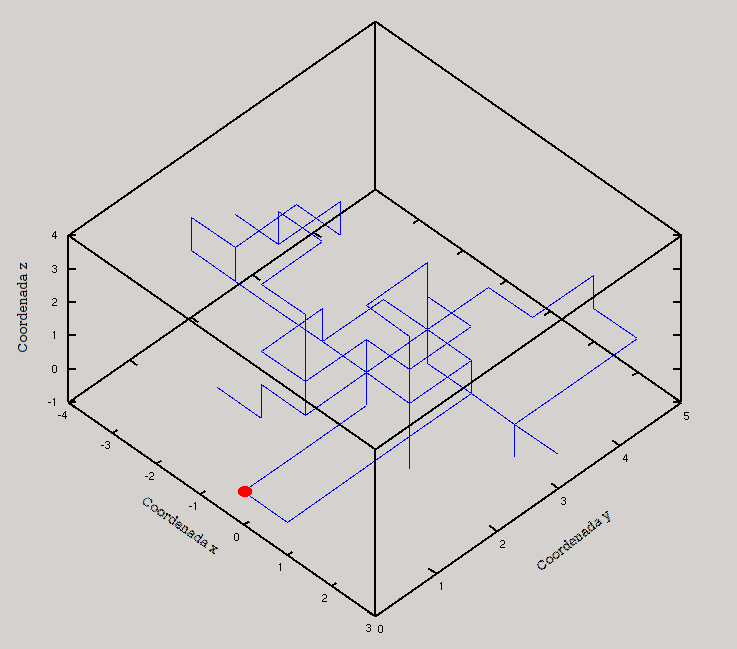
\includegraphics[scale=0.5]{./images/rec3edit.png}
    \caption{Trayectoria de una caminata aleatoria 3D}
  \end{figure}
\end{center} 

\newpage
\section{Apéndice: Código}
Este es el c\'odigo de Octave resuelve una caminata aleatoria de dimensi\'on $dim$ con una cantidad m\'axima de pasos $maxPasos$.
\label{Code1}
\begin{lstlisting}
function M = pasosBorracho(dim, maxPasos)

	M = zeros(dim, 1);
	llego = 0;

	for i = 1:maxPasos
		pos_anterior = M(:,end);
		direccion = floor(rand() * dim)+1;

		delta = 1;
		if rand() < 0.5
			delta = -1;
		endif
		pos_anterior(direccion) += delta;

		M = [M, pos_anterior];

		if pos_anterior == zeros(dim, 1)
			llego = 1;
			break;
		endif
	endfor

	if (llego == 0)
		M = zeros(dim, 1);
	endif
\end{lstlisting}
\label{Code2}
Este c\'odigo genera las caminatas aleatorias para representarlas, teniendo en cuenta que sean lo suficientemente largas como para
que se puede apreciar. 
\begin{lstlisting}
recorrido1 = [];
recorrido2 = [];
recorrido3 = [];

while size(recorrido1) < 30 || size(recorrido1) > 100
	recorrido1 = pasosBorracho(1, 10000);
end

while size(recorrido2) < 30 || size(recorrido2) > 100
	recorrido2 = pasosBorracho(2, 10000);
end

while size(recorrido3) < 30 || size(recorrido3) > 100
	recorrido3 = pasosBorracho(3, 10000);
end

plot(1:size(recorrido1)(2), recorrido1)
plot(recorrido2(1,:), recorrido2(2,:))
plot3(recorrido3(1,:), recorrido3(2,:), recorrido3(3,:))
\end{lstlisting}
\newpage
\label{CodeC}
Este es el c\'odigo en C hace $ITERATIONS$ simulaciones de caminatas aleatorias de dimensi\'on $dim$ con un m\'aximo de pasos
$maxPasos$.
\begin{lstlisting}
#include <stdio.h>
#include <stdbool.h>
#include <stdlib.h>
#include <time.h>

#define MAXPASOS 10000
#define ITERATIONS 10000
#define DIM 1

int pasos[DIM][MAXPASOS];
int anterior[DIM];
bool llego;
int n;

inline int realrand(){
	if (DIM == 3) {
		int a = RAND_MAX;
		while (a >= RAND_MAX - 1) a = rand();
		return a;
	} else {
		return rand();
	}
}

void pasosBorracho(void) {
	llego = false;

	for(int i = 0; i < DIM; i++) {
		pasos[i][0] = 0;
	}

	for(n = 0; !llego && n < MAXPASOS; n++) {
		for(int i = 0; i < DIM; i++) {
			anterior[i] = pasos[i][n];
		}
		int direccion = realrand()%DIM;
		int delta = 1;
		if (realrand() % 2)
			delta = -1;

		anterior[direccion] += delta;

		for(int i = 0; i < DIM; i++) 
			pasos[i][n+1] = anterior[i];
		
		bool yallego = true;
		for (int i = 0; yallego && i < DIM; i++)
			if (anterior[i] != 0)
				yallego = false;
		
		if (yallego)
			llego = true;
	}
}

int main() {

	srand(time(NULL));

	for(int i = 0; i < ITERATIONS; i++) {
		pasosBorracho();
		if (n != MAXPASOS) {
			for(int i = 0; i <= n; i++)  {
				for (int j = 0; j < DIM; j++) {
					printf("%d ", pasos[j][i]);
				}
				printf("\n");
			}
		} else {
			printf("0\n");
		}
		printf("\n");
	}
}
\end{lstlisting}
\label{CodePy}
Este c\'odigo en Python hace la transformación de la soluci\'on creada por los programas hechos en C a un vector columna, que Octave puede abrir, con la cantidad de pasos que tomó cada caminata.
\begin{lstlisting}
if __name__ == '__main__':

	input = raw_input("Input file: ")
	output = raw_input("Output file: ")

	e = open(input, 'r').readlines()
	sizes = []
	n = 0

	for i in e:
		if i == '\n':
			if n != 0:
				sizes.append(n)
			n = 0
		else:
			n += 1
	
	f = open(output, 'w')
	
	for i in sizes:
		f.write('%d\n'%i)

	f.close()
\end{lstlisting}
\label{Code3}
Este fragmento de c\'odigo en Octave hace las simulaciones y estima la probabilidad de la vuelta a casa y el promedio de pasos
hasta la vuelta.
\begin{lstlisting}
f = input("Filename: ", "s");
s = load(f);
v = []

for i=1:size(s)(1)
	if s(i) != 1
		v = [v, s(i)];
	end
end

printf("De 10000, solo %d volvieron al inicio\n", size(v)(2));
printf("Promedio de pasos necesarios: %f\n", sum(v)/size(v)(2));

bar(hist(v, [1, 5, 25, 625, 10000]))
\end{lstlisting}
\end{document}
